\documentclass[handout]{beamer}

\usepackage{fontspec} 
\usepackage{lsp-makros}
\useoutertheme{lsp}

\usepackage{lsptitle}

\def\two@digits#1{\ifnum#1<10 0\fi\number#1}
\def\mytoday{\two@digits{\number\day}.\two@digits{\number\month}.\number\year}


\usepackage{xspace,multicol}
\newcommand{\latex}{\LaTeX\xspace}
\usepackage{tikz}


\newcounter{lastpagemainpart}
\footnotesep0pt
\renewcommand{\footnoterule}{}
\usefootnotetemplate{
  \noindent
  \insertfootnotemark\insertfootnotetext}

\let\beamerfn=\footnote
\renewcommand{\footnote}[1]{%
\let\oldfnsize=\footnotesize%
\let\footnotesize=\tiny%
\beamerfn<\thebeamerpauses->{#1}%
\let\footnotesize=\oldfnsize}


\date{\today}

\usepackage{eurosym}  
 
\renewcommand{\centerline}[1]{\hfill#1\hfill\hfill\mbox{}}


\title{Titel}
% \institute{FU Berlin}
\author[LangSci]{Author Name}



\begin{document}
 
\frame{
\frametitle{\mbox{Language Science Press + Cross Linguistic Linked Data }}
\begin{tabular}{p{5cm}p{5cm}}
\parbox{5.5cm}{
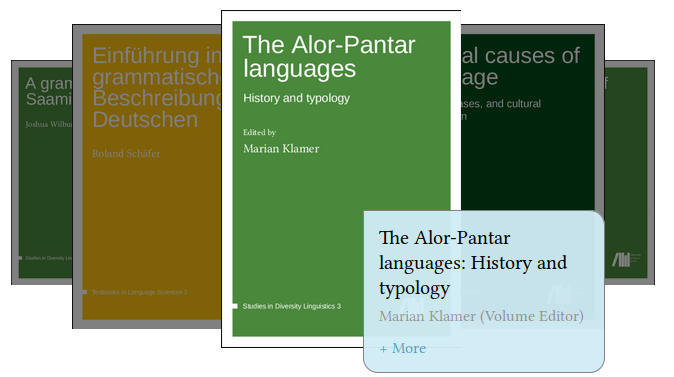
\includegraphics[width=5cm]{catalog.png}
}
&
\parbox{5cm}{
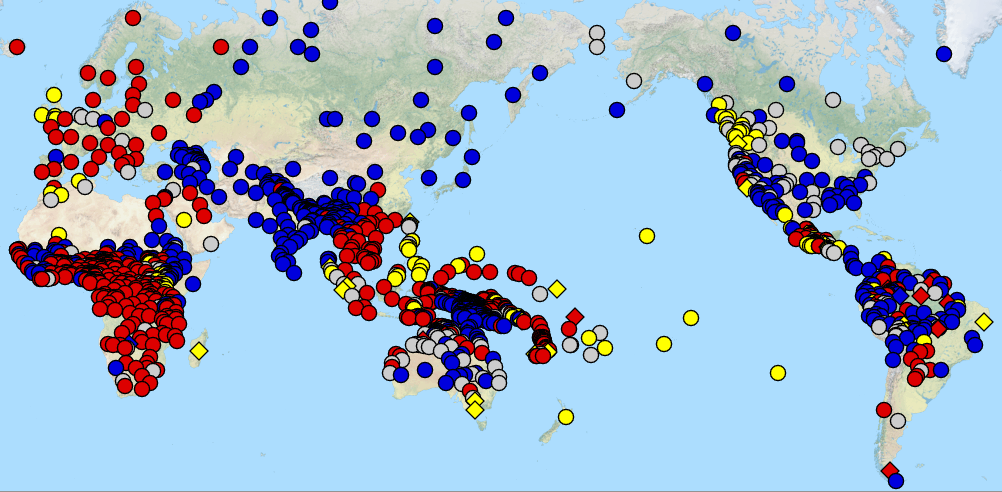
\includegraphics[width=5.5cm]{wals-sov.png}
}
\\\\
\parbox{5.5cm}{
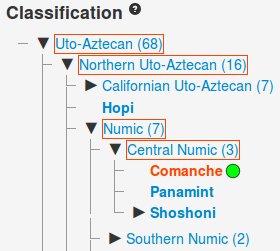
\includegraphics[width=5cm]{comanche.png}
}&
\parbox{5.5cm}{
\begin{itemize}
 \item 10$^4$ linguistische Beispiele
 \item 10$^5$ typologische Datenpunkte
 \item 25\,000 Sprachen/Dialekte, 265\,000 Literaturangaben
 \item CSV, XML, bib, RDF
 \item CC-BY(-SA)
\end{itemize}
\bigskip	
}
\end{tabular}

} 

\end{document}